\documentclass[11pt,a4paper]{article}
\usepackage{fontspec}
\setmainfont{TeX Gyre Pagella}
\newfontfamily\headfont{Inter}[UprightFont=*-ExtraBold,BoldFont=*-ExtraBold,Extension=.otf,Path=/usr/share/fonts/opentype/inter/]
\usepackage[a4paper,margin=2.3cm]{geometry}
\usepackage{graphicx,booktabs,float,caption,array,xcolor,longtable}
\usepackage{xurl}
\usepackage[hidelinks]{hyperref}
\usepackage{titlesec}
\usepackage[round]{natbib}
\usepackage{setspace}
\setstretch{1.05}
\renewcommand{\topfraction}{0.9}
\renewcommand{\bottomfraction}{0.8}
\renewcommand{\textfraction}{0.1}
\renewcommand{\floatpagefraction}{0.75}
\setlength{\parindent}{0pt}
\setlength{\parskip}{0.55em}
\titleformat{\section}{\headfont\Large}{\thesection}{0.8em}{}
\titleformat{\subsection}{\headfont\large}{\thesubsection}{0.8em}{}
\captionsetup{font=small,labelfont=bf}
\urlstyle{same}
\hypersetup{pdftitle={Pirate Hotspots, Then and Now},pdfauthor={Tristan Hotham}}

\begin{document}
\begin{center}
{\Large\bfseries Pirate Hotspots, Then and Now\par}
\vspace{0.4em}
{\large How maritime piracy moved around the world:\\7,511 mapped attacks, 1993 to 2020, and IMB counts to 2026\par}
\vspace{1.2em}
{\large Tristan Hotham\par}
\vspace{0.3em}
{\small Independent researcher\\
ORCID: 0000-0003-4931-9349\\
DOI: https://doi.org/10.5281/zenodo.23856383\par}
\vspace{0.8em}
2026
\end{center}

\begin{quote}
\small
\begin{center}\textbf{Abstract}\end{center}
Maritime piracy is often pictured through one episode, the Somali hijackings of the late 2000s, but its geography has shifted repeatedly. Using the Crime at Sea database of 7,511 geolocated attacks and attempted attacks from 1993 to 2020, compiled from International Maritime Bureau (IMB) and US National Geospatial-Intelligence Agency reports, I map piracy year by year and trace how its hotspots moved. In the 1990s the South China Sea and East Asian waters led (26\% of attacks in 1993 to 1999), followed by Indonesia, which peaked at 105 attacks in 2003. The Strait of Malacca peaked at 104 attacks in 2000 and averaged 14.3 a year from 2006. Attacks in Somali waters and the Gulf of Aden rose from 53 in 2007 to 231 in 2011, making up 48\% of all attacks and 83\% of hijackings in 2008 to 2011, with a median distance from shore of 131 km against 9.1 km elsewhere in those years, and then fell by 92\% in two years. The Gulf of Guinea became the leading region, with 43\% of attacks in 2020. IMB headline counts carry the story to 2026: the Singapore Strait recorded 80 incidents in 2025, 58\% of the world total, and all 8 hijackings reported in January to September 2026 were by Somali pirates. Most attacks are thefts from ships at anchor close to shore, in busy shipping lanes and in poorer countries; the hotspots move with enforcement, opportunity and the routes of trade.

\textbf{Keywords:} maritime piracy; armed robbery at sea; Somalia; Strait of Malacca; Singapore Strait; Gulf of Guinea; IMB; spatial analysis; shipping density; open data
\end{quote}

\section{Introduction}
Piracy, and the armed robbery against ships that the IMB counts alongside it, is one of the oldest crimes at sea and one of the best recorded. Since 1991 the IMB Piracy Reporting Centre in Kuala Lumpur has collected reports from shipmasters and owners and published them in quarterly and annual reports \citep{imb}. The US National Geospatial-Intelligence Agency publishes a parallel series of Anti-Shipping Activity Messages \citep{asam}. Researchers have turned these reports into event datasets to study the causes of piracy \citep{coggins,daxecker} and the effect of counter-piracy measures \citep{shortland,bueger}.

This paper asks a simpler, descriptive question: where has piracy happened, and how have its hotspots moved, from 1993 to today? It uses an open, geolocated database of 7,511 attacks \citep{benden}, the IMB's headline counts for 2021 to 2026, and a global map of ship traffic \citep{wbships}, and is accompanied by an interactive map with a year slider (\url{https://maps.tristanhotham.com/piracy-hotspots/}).

\section{Data}
\textbf{Attacks, 1993 to 2020.} The Crime at Sea database \citep{benden} gives 7,511 attacks with a date, latitude and longitude, attack type (attempted, boarded, hijacked and, from 2015, fired upon), the state of the ship (anchored, berthed or steaming), vessel name, the nearest country and the country whose exclusive economic zone (EEZ) contains the position, and the distance to the nearest shore. Records for 1993 to 2014 (6,338) come from the MAPPING piracy data compiled by Brandon Prins from IMB and ASAM reports; records for 2015 to 2020 (1,173) were taken from IMB reports and include the IMB's narrative. I used the copy published on GitHub with the paper (CC BY 4.0).

\textbf{IMB headline counts, 2021 to 2026.} The database ends in 2020. For later years I transcribed the headline numbers from the IMB's annual reports and press releases: world totals for 2021 to 2025 and for January to September 2025 and 2026, and, where the releases give them, incidents in the Singapore Strait, Indonesia and the Gulf of Guinea, hijackings and crew taken hostage or kidnapped (Table~\ref{tab:imb}). These are not geolocated and are kept separate in every figure.

\textbf{Shipping density.} The World Bank and IMF Global Shipping Traffic Density raster counts AIS positions from January 2015 to February 2021 \citep{wbships,cerdeiro}. I used the 0.08 degree overview of the all-vessels layer. Because the overview subsamples the full-resolution raster, I use it only averaged over 1 degree squares (about 144 samples each).

\textbf{Country indicators and geography.} The database comes with yearly country indicators, including GDP per person and the Corruption Perceptions Index, which I use only descriptively. Outlines are from Natural Earth \citep{naturalearth}.

\section{Methods}
\textbf{Attack types.} The source codes boardings as ``Boarded'' in some years and ``Boarding'' in others; I merged them. ``Fired upon'' appears 3 times before 2015 and 70 times from 2015, so earlier ships fired upon but not boarded are mostly coded as attempted; the 101 attacks of 1993 have no type.

\textbf{Regions.} Each attack is assigned to one region by the first rule that applies: the Singapore Strait (a box from 103.42 to 104.65$^\circ$E and 0.85 to 1.60$^\circ$N, including the Batam and Bintan anchorages); the Strait of Malacca (a polygon from the Andaman Sea entrance to the western end of the Singapore Strait); Indonesian waters (nearest country or EEZ Indonesia or Timor-Leste); the South China Sea, Philippines and East Asia; the Indian subcontinent (within 300 km of India, Bangladesh, Sri Lanka, Pakistan or the Maldives); the East African coast (within 60 km of Kenya to South Africa, Madagascar and the Comoros); Somali waters (everything else between 32 and 80$^\circ$E and 15$^\circ$S and 30$^\circ$N, outside the Persian Gulf, which includes the Gulf of Aden, the southern Red Sea, the Somali Basin and the Arabian Sea); the Gulf of Guinea and West Africa (30$^\circ$W to 16$^\circ$E, 20$^\circ$S to 20$^\circ$N); the Americas; and elsewhere. Table~\ref{tab:regions} gives the totals.

\textbf{Eras and hotspots.} I divide the period into six eras that follow the main shifts: 1993 to 1999, 2000 to 2004, 2005 to 2007, 2008 to 2011, 2012 to 2015 and 2016 to 2020. Hotspots are 1 degree squares, named from the location descriptions of the attacks in them. The maps use hexagons about 4 degrees across.

\textbf{Distance from shore and traffic.} Distances are the source's great-circle distances to the nearest coast. For traffic, I rank all 1 degree squares with any AIS traffic (31,455) by mean density and record the percentile of the square each attack fell in.

\section{Results}
\subsection{Totals}
Reported attacks rose from 95 in 1994 to 469 in 2000, stayed above 236 a year until 2011, and fell to 190 in 2020 (Figure~\ref{fig:years}). The IMB counted 132 incidents in 2021, 115 in 2022, 120 in 2023, 116 in 2024 and 137 in 2025, and 51 in January to September 2026. The IMB's 2022 total is 75\% below the database's 2000 peak.

\begin{figure}[tbp]\centering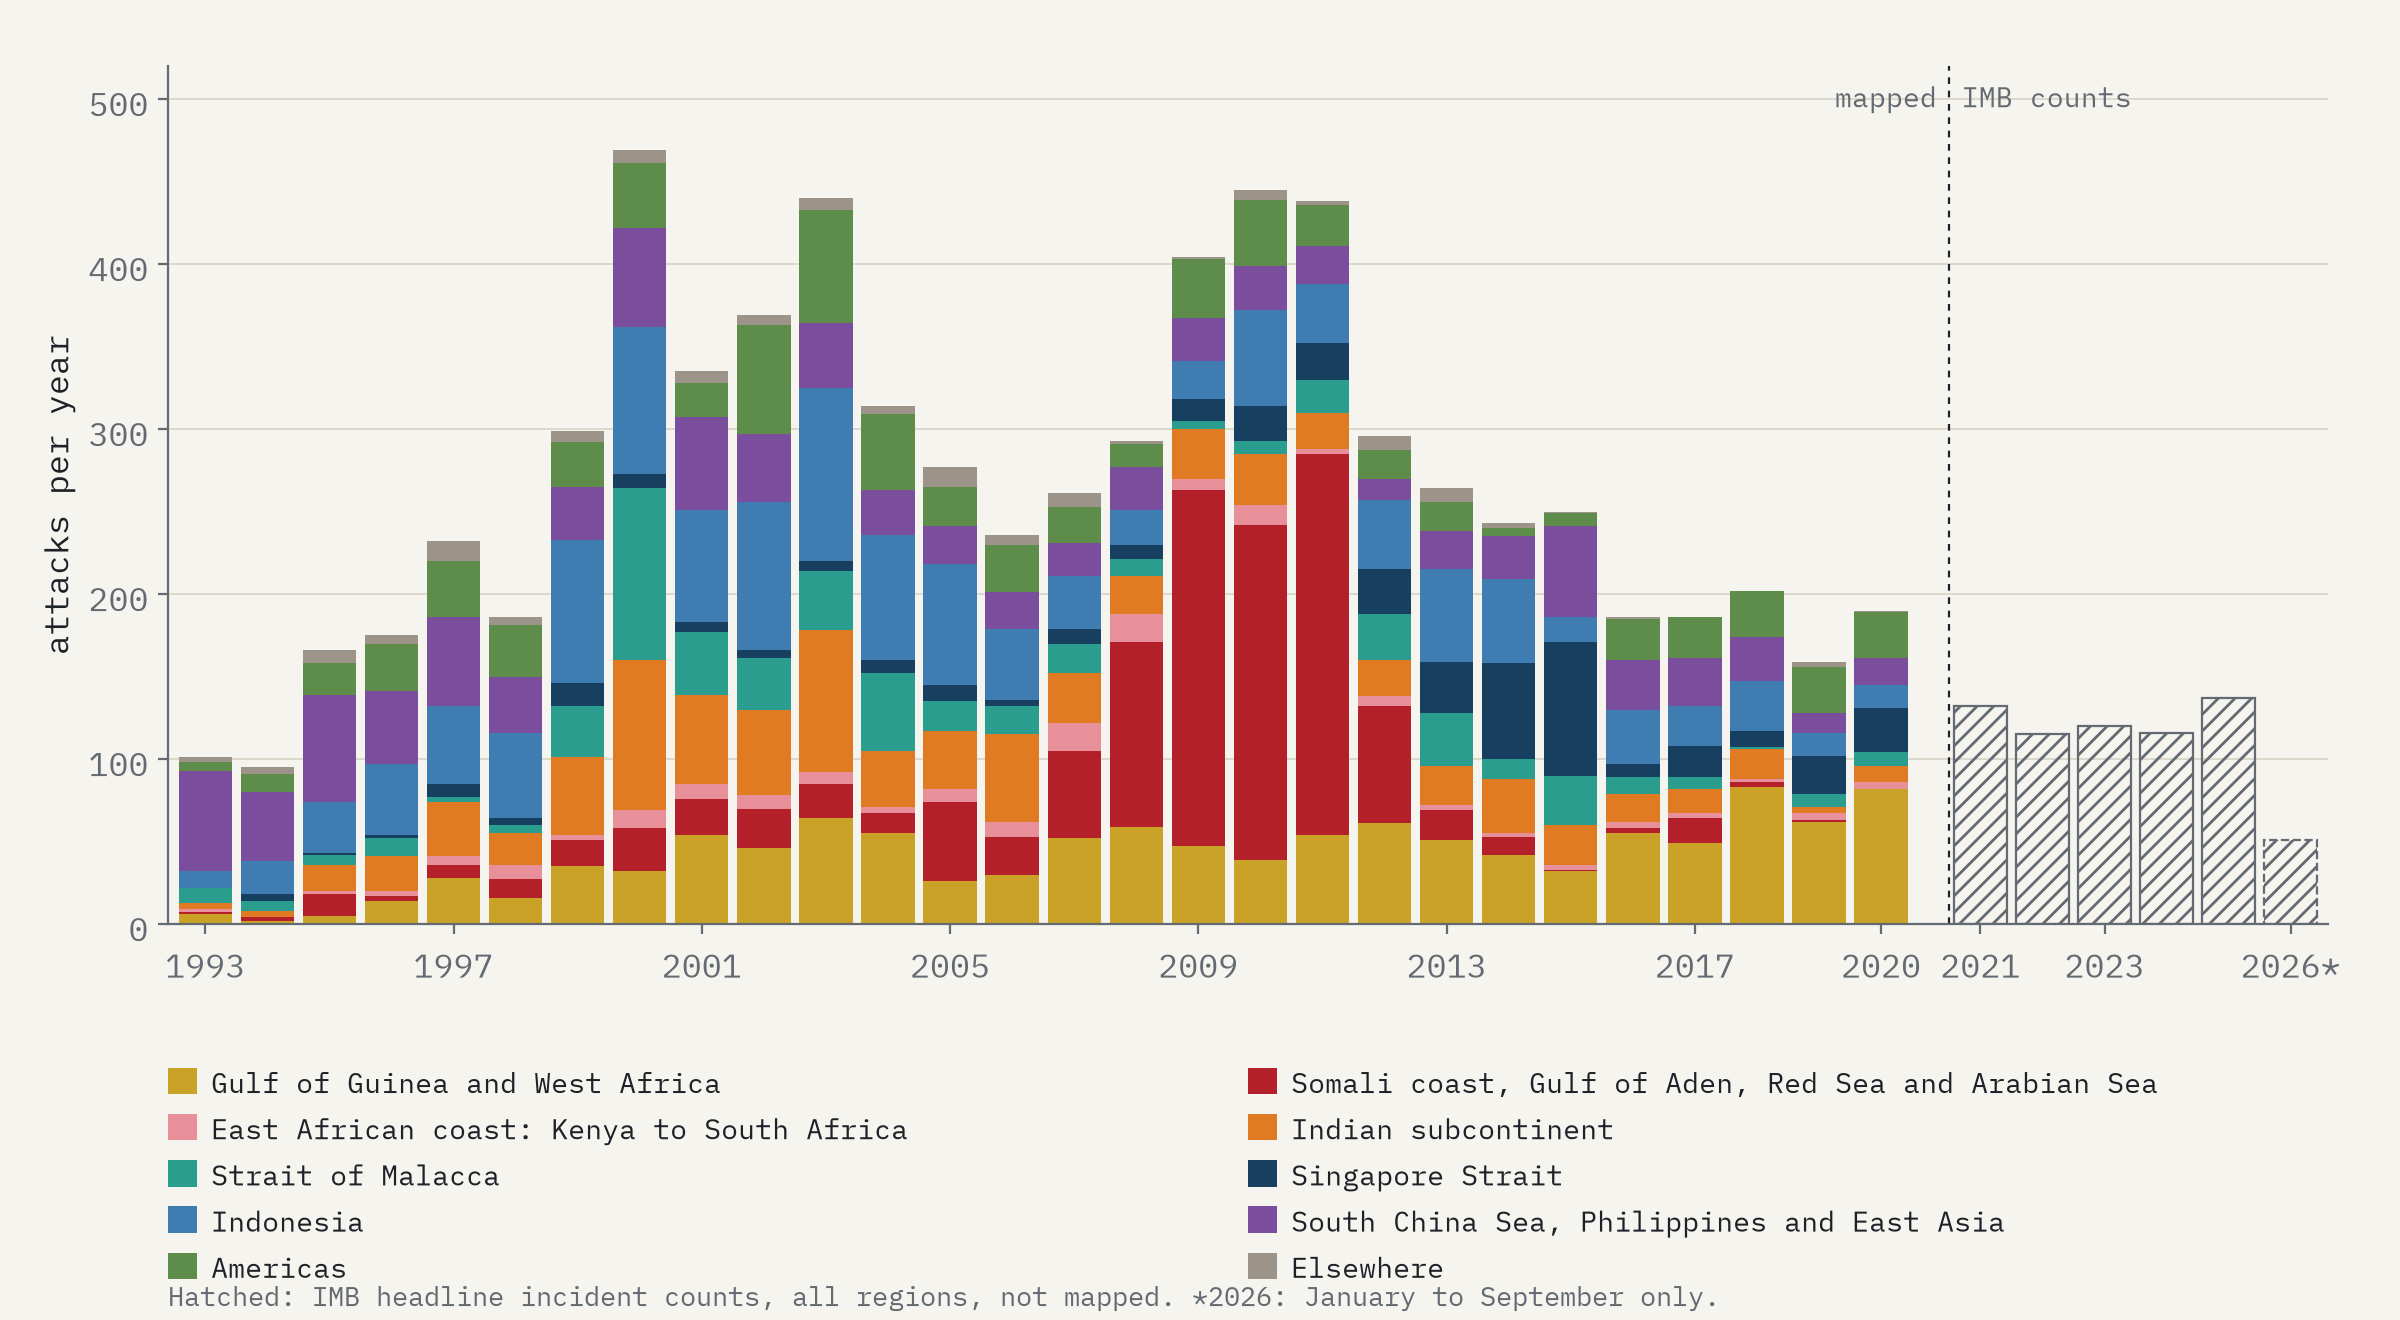
\includegraphics[width=\textwidth]{f_years.png}
\caption{Attacks per year by region, 1993 to 2020 (Crime at Sea database), and IMB headline incident counts for all regions, 2021 to 2025 and January to September 2026 (hatched).}\label{fig:years}\end{figure}

\begin{table}[tbp]\centering\small\caption{Attacks by region, 1993 to 2020: total, share, peak year (attacks), median distance from shore and share hijacked.}\label{tab:regions}\begin{tabular}{p{6.2cm}rrrrr}\toprule Region & Attacks & Share & Peak year & Median km & Hijacked\\\midrule
Gulf of Guinea and West Africa & 1,181 & 15.7\% & 2018 (83) & 10.0 & 5\%\\
Somali coast, Gulf of Aden, Red Sea and Arabian Sea & 1,168 & 15.6\% & 2011 (231) & 110.5 & 20\%\\
East African coast: Kenya to South Africa & 167 & 2.2\% & 2007 (17) & 2.4 & 1\%\\
Indian subcontinent & 852 & 11.3\% & 2000 (91) & 5.0 & 1\%\\
Strait of Malacca & 559 & 7.4\% & 2000 (104) & 9.4 & 7\%\\
Singapore Strait & 439 & 5.8\% & 2015 (81) & 9.5 & 4\%\\
Indonesia & 1,283 & 17.1\% & 2003 (105) & 10.9 & 3\%\\
South China Sea, Philippines and East Asia & 953 & 12.7\% & 1995 (65) & 10.1 & 8\%\\
Americas & 769 & 10.2\% & 2003 (69) & 2.4 & 1\%\\
Elsewhere & 140 & 1.9\% & 1997 (12) & 8.6 & 10\%\\
\bottomrule\end{tabular}\end{table}

\subsection{How the hotspots moved}
Figure~\ref{fig:eras} shows the six eras side by side and Table~\ref{tab:hotspots} the busiest squares in each.

\textbf{1993 to 1999: the South China Sea and Indonesia.} The South China Sea, Philippines and East Asian waters had 332 attacks (26\%), led by waters off China and Hong Kong and around the Philippines; Indonesia had 290 and overtook them in 1998. Across 1993 to 2004 the waters of Southeast and East Asia, including the two straits, held 52\% of all attacks. The busiest squares were anchorages: Jakarta and Tanjung Priok, Chittagong and Belawan.

\textbf{2000 to 2004: the Strait of Malacca.} The Malacca Strait peaked at 104 attacks in 2000 and averaged 51.2 a year in 2000 to 2004. It then fell to 18 in 2005 and averaged 14.3 a year from 2006 to 2020 (3.6 times lower), never above 32. The fall followed coordinated naval patrols by Indonesia, Malaysia and Singapore from 2004 and joint air patrols from 2005, and the 2004 tsunami, which devastated the Aceh coast \citep{liss}. Indonesia peaked in 2003 with 105. The Indian subcontinent peaked in 2000 with 91; the Chittagong anchorages are the busiest square of the whole record (366 attacks).

\textbf{2008 to 2011: Somalia.} Attacks in Somali waters rose from 53 in 2007 to 231 in 2011: 762 in four years, 48\% of all attacks. They included 163 of the world's 197 hijackings. 99\% were against ships under way and 73\% were attempts that failed. Their spread across the Gulf of Aden, the Somali Basin and the Arabian Sea means that only two Gulf of Aden squares appear among the five busiest of the era. They fell to 71 in 2012, 18 in 2013 and 23 in all of 2015 to 2020, after international naval patrols, armed security teams on ships, industry best management practices and action against pirate groups ashore \citep{worldbank,bueger,shortland}. From 2014 to 2020 there were 3 hijackings in these waters, all in 2017.

\textbf{2012 to 2015: the Singapore Strait.} With fewer than 6.2 attacks a year on average to 2008, the Singapore Strait rose to 81 in 2015 and led the world in this era (197 attacks). 89\% of its attacks in 2014 and 2015 were boardings. It fell to 8 in 2016.

\textbf{2016 to 2020: the Gulf of Guinea.} The Gulf of Guinea and West Africa rose from 8\% of attacks in the 1990s to 36\% in 2016 to 2020, peaking at 83 in 2018 with 82 in 2020 (43\% of the world). The median distance from shore rose from 7.2 km before 2016 to 23.2 km, 80 attacks were more than 50 nautical miles out, and 60 of the 331 IMB narratives mention kidnapping. 49 of the 69 ships fired upon in these years were in the region.

\begin{figure}[tbp]\centering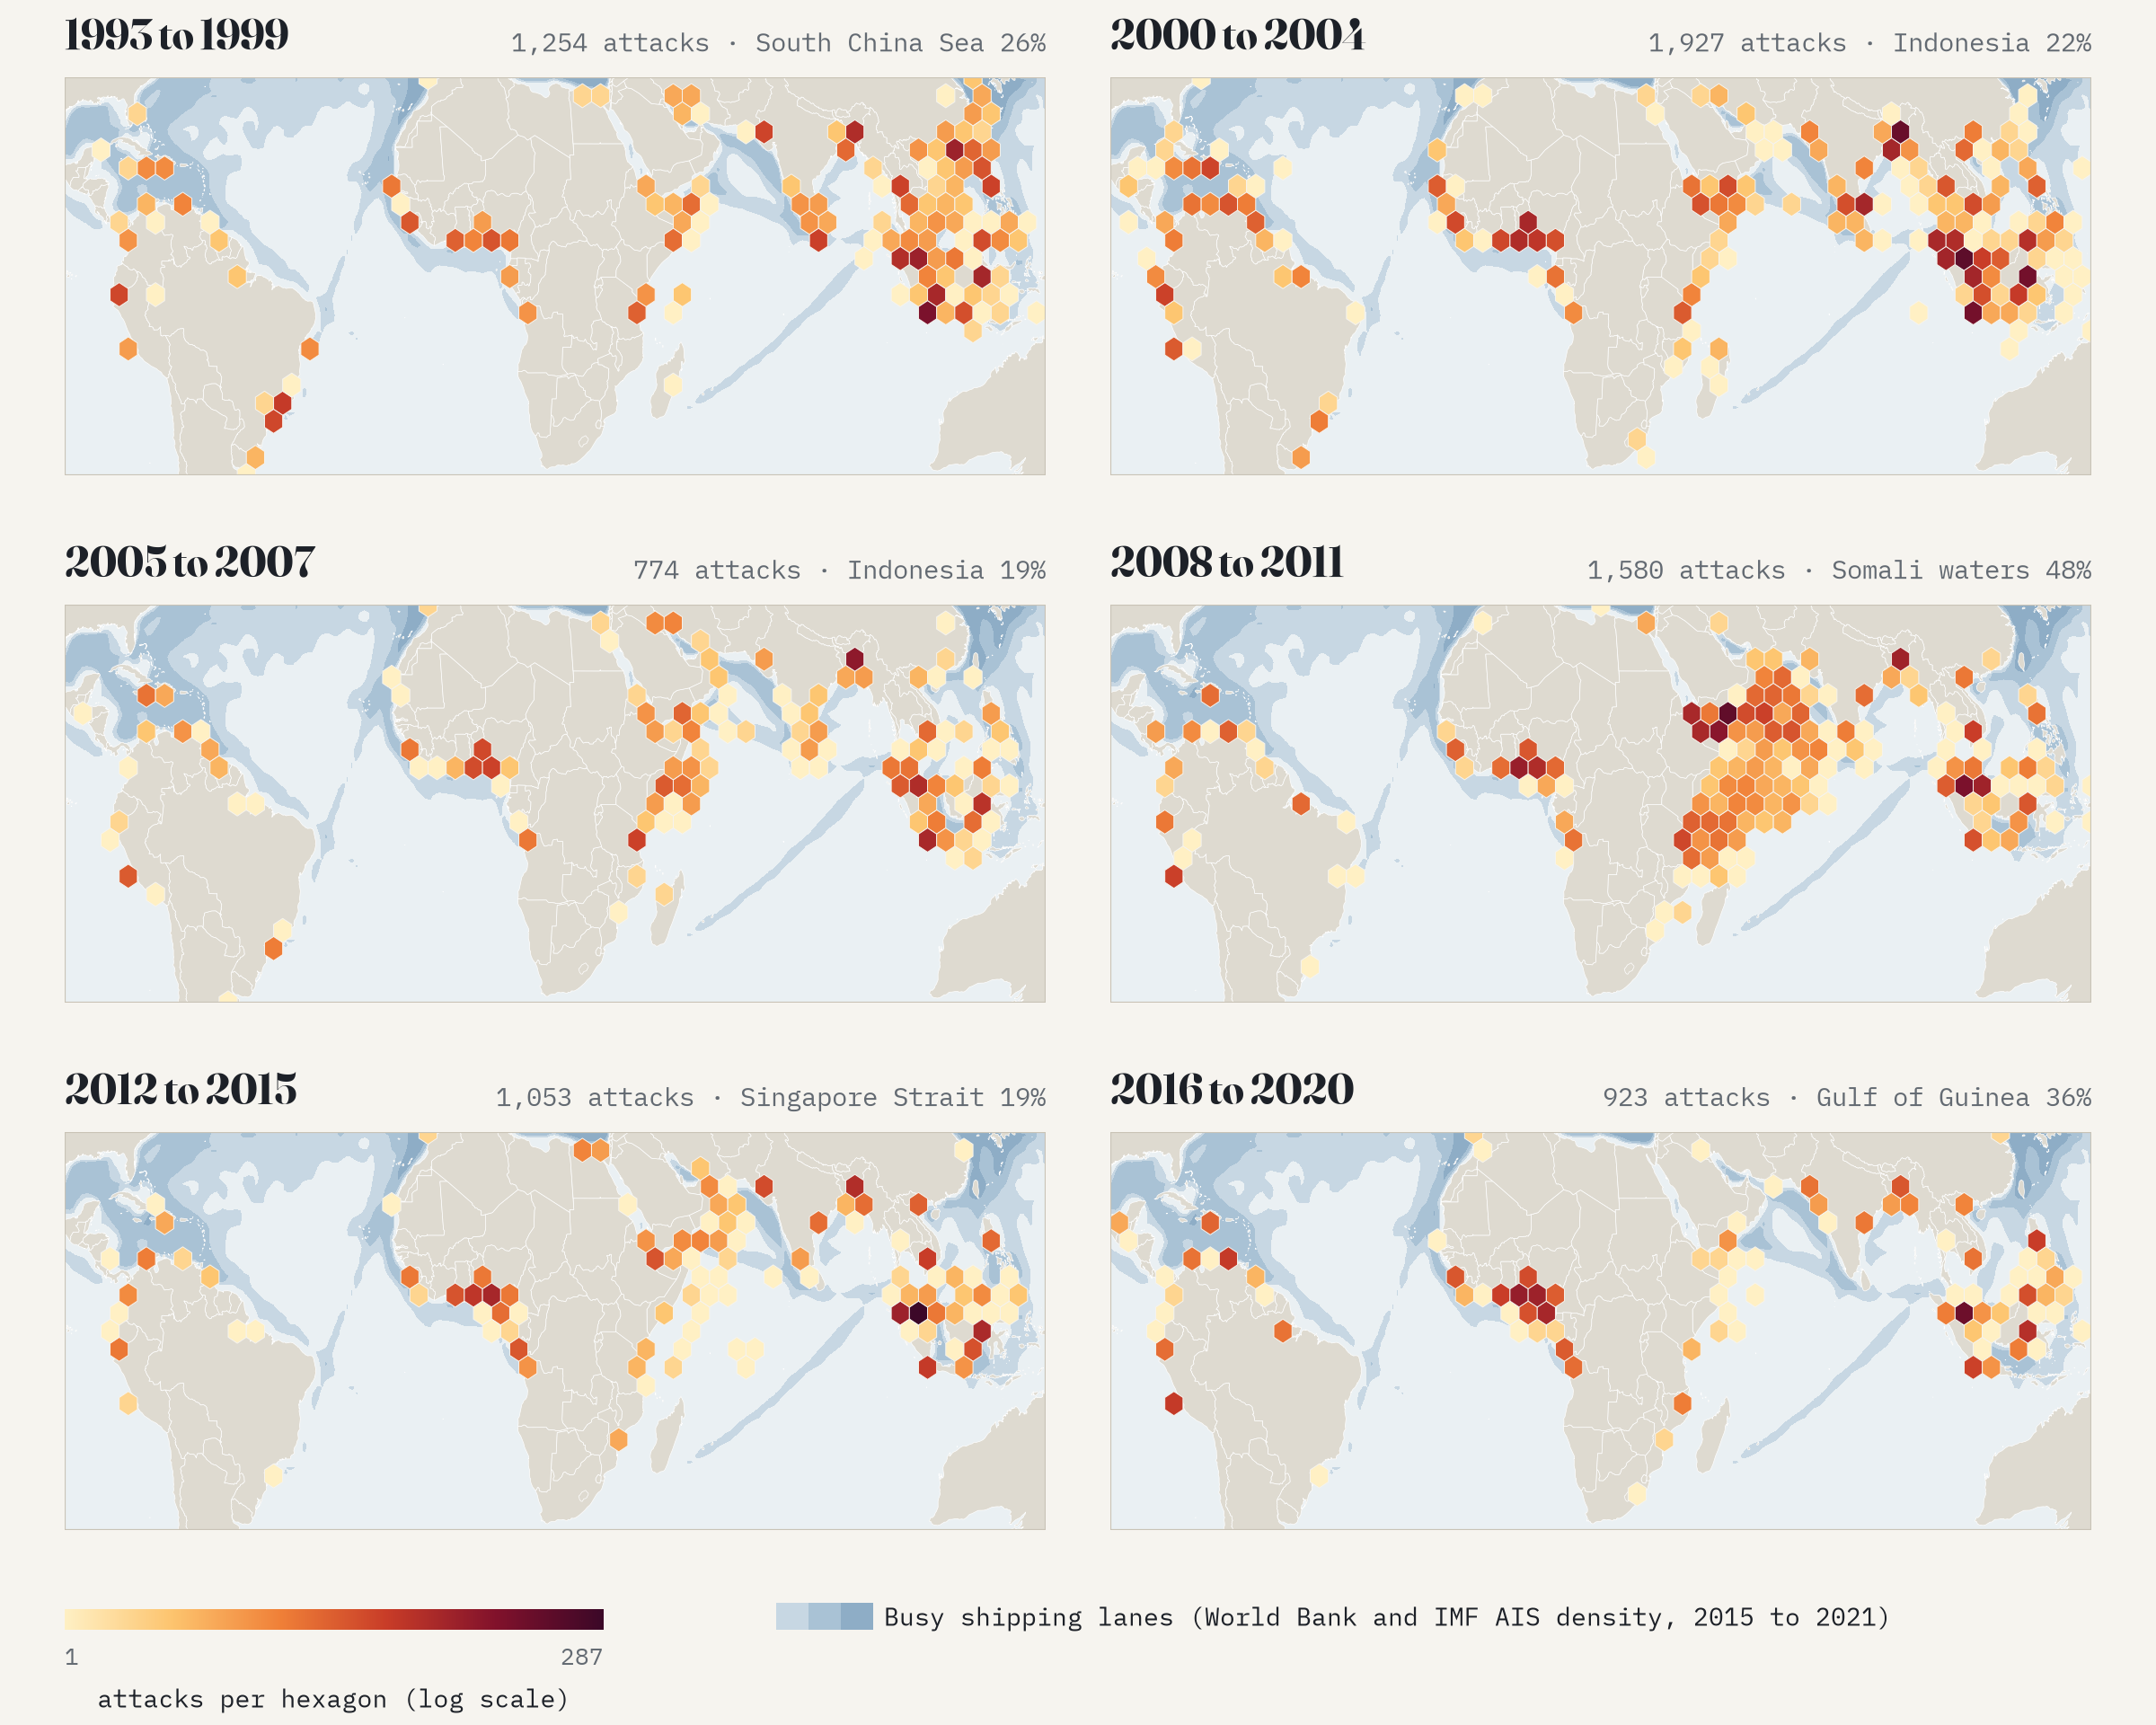
\includegraphics[width=\textwidth]{f_eras.png}
\caption{Attacks by era, counted in hexagons about 4 degrees across (one colour scale for all panels), over the busiest shipping lanes (World Bank and IMF AIS density, 2015 to 2021, smoothed at 1 degree).}\label{fig:eras}\end{figure}

\begin{table}[tbp]\centering\small\caption{The five busiest 1 degree squares in each era, with their share of the era's attacks.}\label{tab:hotspots}\begin{tabular}{llrr}\toprule Era & Square & Attacks & Share\\\midrule
1993 to 1999 & Jakarta and Tanjung Priok, Indonesia & 45 & 3.6\%\\
 & Chittagong anchorages, Bangladesh & 44 & 3.5\%\\
 & Belawan, Sumatra, Indonesia & 39 & 3.1\%\\
 & Gelasa Strait and Bangka, Indonesia & 34 & 2.7\%\\
 & Hong Kong waters & 33 & 2.6\%\\
\addlinespace
2000 to 2004 & Chittagong anchorages, Bangladesh & 128 & 6.6\%\\
 & Lagos anchorages, Nigeria & 74 & 3.8\%\\
 & Jakarta and Tanjung Priok, Indonesia & 65 & 3.4\%\\
 & Balikpapan, Indonesia & 60 & 3.1\%\\
 & Malacca Strait off Tanjung Tohor & 60 & 3.1\%\\
\addlinespace
2005 to 2007 & Chittagong anchorages, Bangladesh & 74 & 9.6\%\\
 & Lagos anchorages, Nigeria & 42 & 5.4\%\\
 & Jakarta and Tanjung Priok, Indonesia & 29 & 3.7\%\\
 & Dar es Salaam, Tanzania & 25 & 3.2\%\\
 & Balikpapan, Indonesia & 20 & 2.6\%\\
\addlinespace
2008 to 2011 & Chittagong anchorages, Bangladesh & 58 & 3.7\%\\
 & Gulf of Aden, central & 52 & 3.3\%\\
 & Lagos anchorages, Nigeria & 51 & 3.2\%\\
 & Singapore Strait, eastern part & 44 & 2.8\%\\
 & Gulf of Aden, west of centre & 40 & 2.5\%\\
\addlinespace
2012 to 2015 & Singapore Strait, western part & 129 & 12.3\%\\
 & Singapore Strait, eastern part & 109 & 10.4\%\\
 & Belawan, Sumatra, Indonesia & 54 & 5.1\%\\
 & Chittagong anchorages, Bangladesh & 42 & 4.0\%\\
 & Dumai, Sumatra, Indonesia & 29 & 2.8\%\\
\addlinespace
2016 to 2020 & Singapore Strait, eastern part & 64 & 6.9\%\\
 & Lagos anchorages, Nigeria & 57 & 6.2\%\\
 & Niger Delta offshore, Nigeria & 38 & 4.1\%\\
 & Samarinda and Muara Berau, Indonesia & 38 & 4.1\%\\
 & Singapore Strait, western part & 35 & 3.8\%\\
\addlinespace
\bottomrule\end{tabular}\end{table}

\subsection{What kind of attack}
64\% of all attacks were boardings, 27\% attempts, 7\% hijackings (511, peaking at 53 in 2010) and 1.0\% ships fired upon (Figure~\ref{fig:types}). Where the ship's state is known, 60\% were at anchor or berthed. Boardings were 43\% of attacks in 2008 to 2011, when Somali attempts were common, and 76\% in 2016 to 2020.

\begin{figure}[tbp]\centering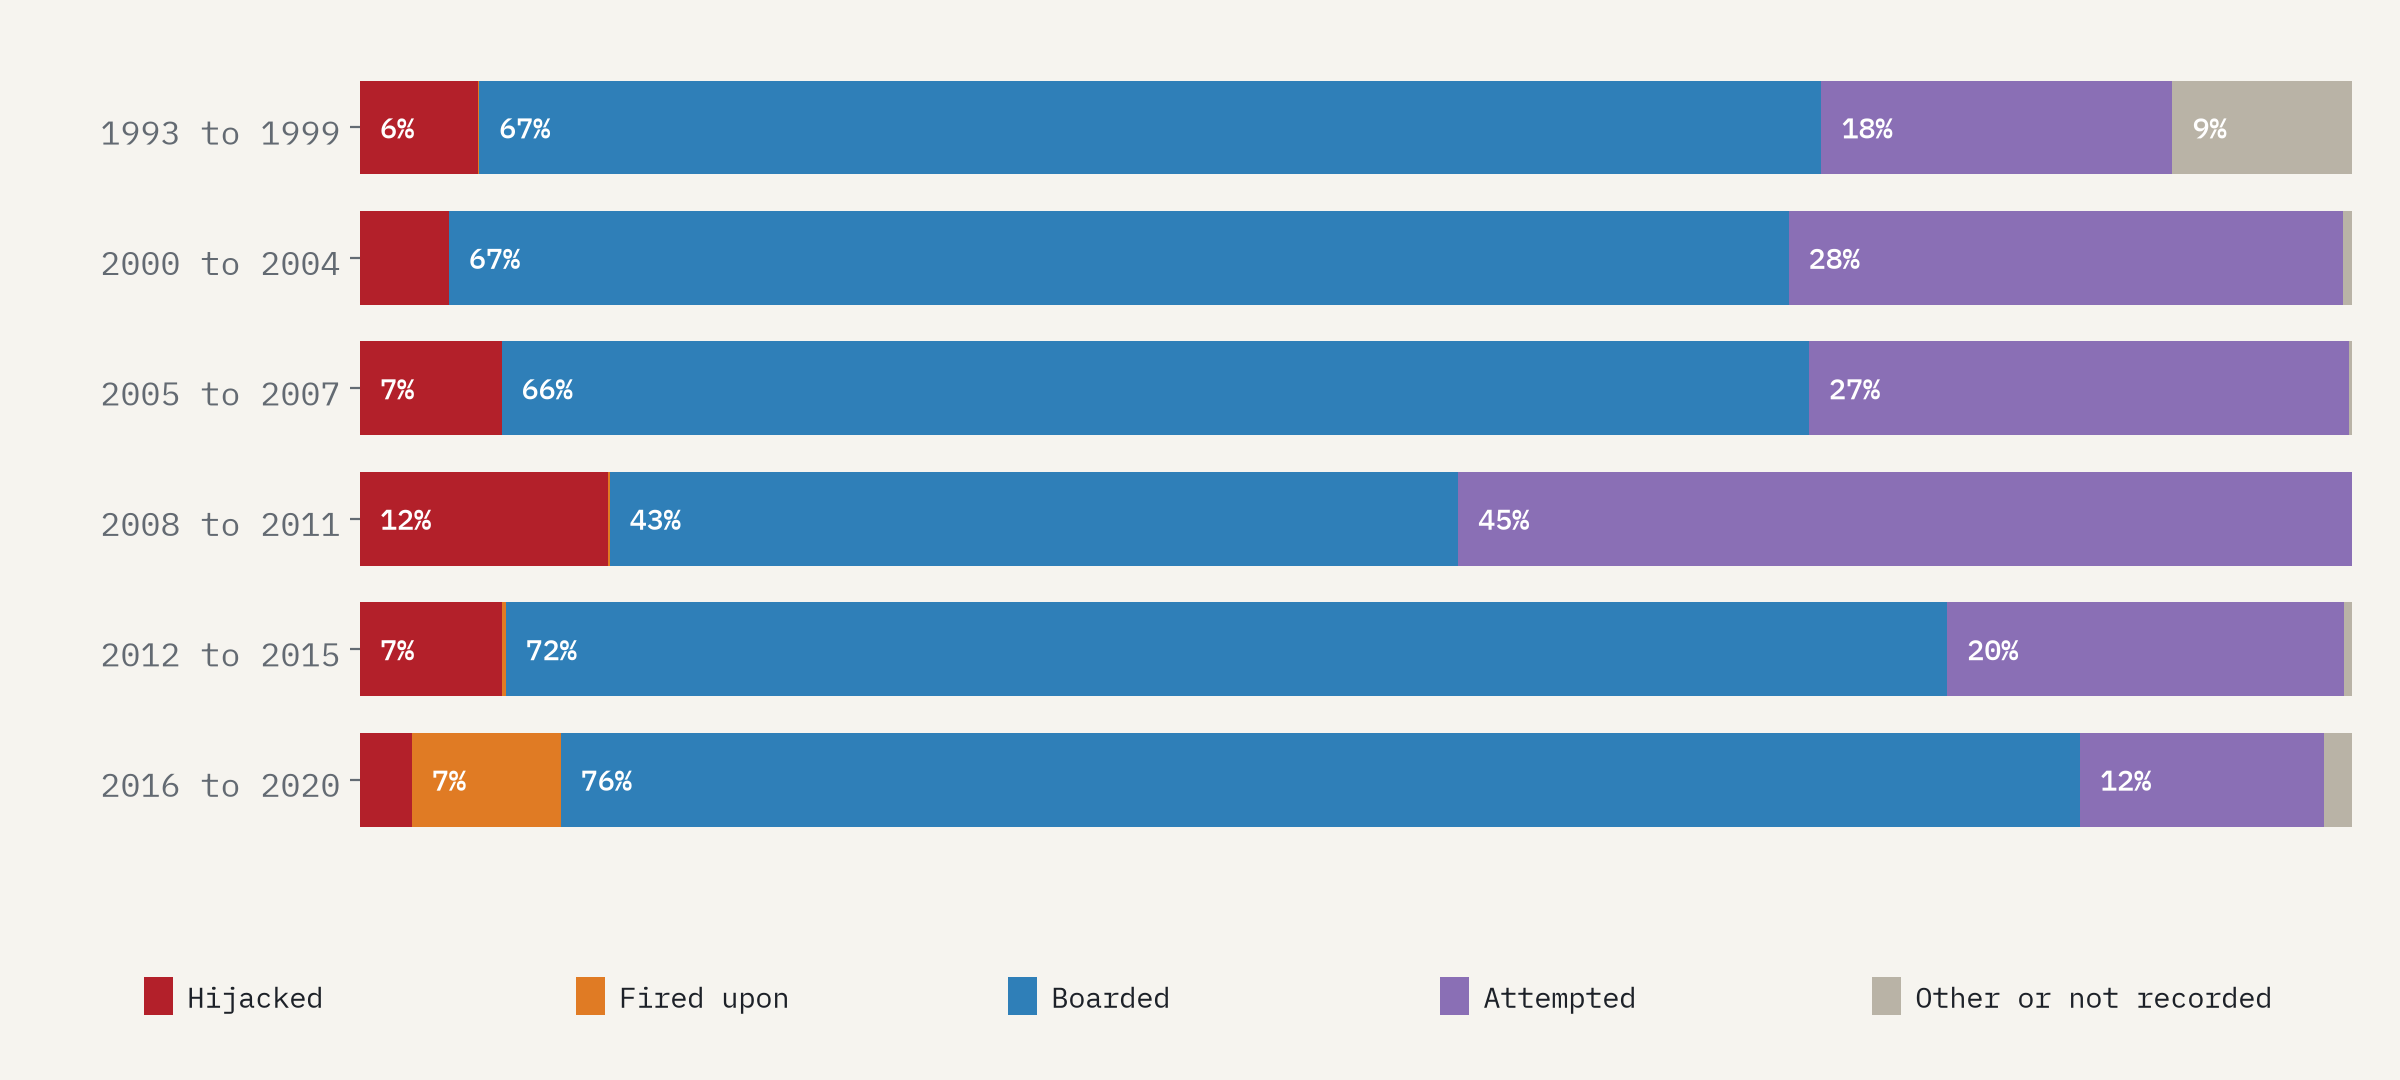
\includegraphics[width=\textwidth]{f_types.png}
\caption{Attack types by era. ``Fired upon'' is recorded almost only from 2015.}\label{fig:types}\end{figure}

\subsection{Distance from shore}
The median attack was 10.1 km from shore and 65\% were within 20 km; ships at anchor were attacked a median 5.2 km out and ships under way 42.0 km out (Figure~\ref{fig:shore}). Somali waters are the exception: a median 131 km in 2008 to 2011, 204 km in 2010, with 41\% beyond 100 nautical miles. Of the 542 attacks that far out (7.2\% of all), 72\% were in Somali waters.

\begin{figure}[tbp]\centering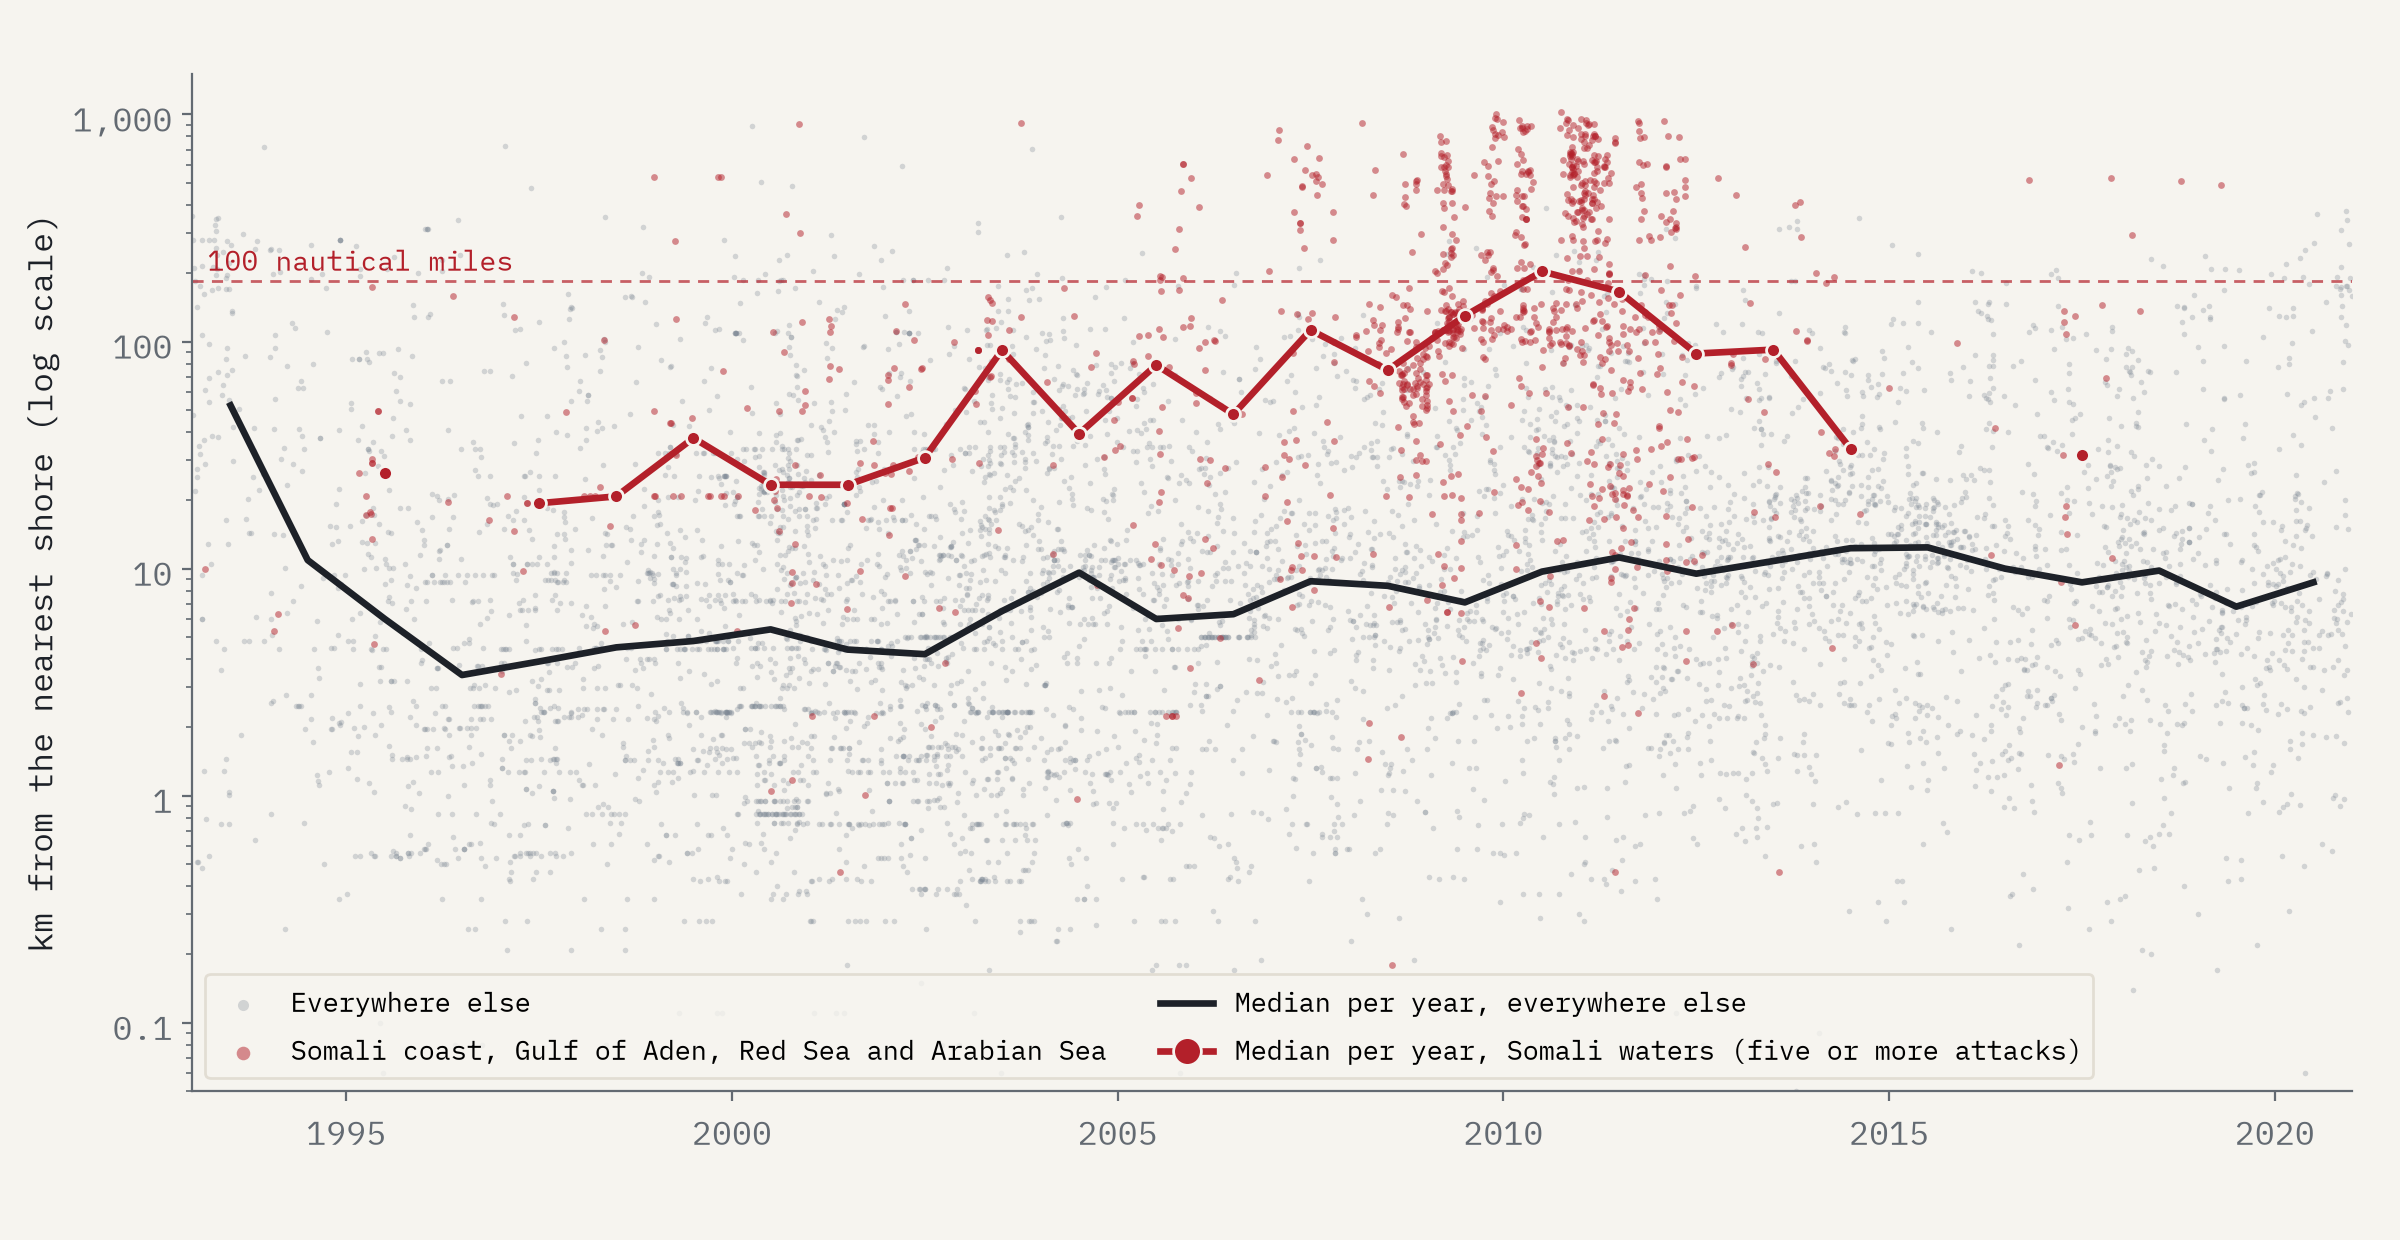
\includegraphics[width=\textwidth]{f_shore.png}
\caption{Distance from the nearest shore of every attack, with yearly medians for Somali waters (years with five or more attacks) and everywhere else.}\label{fig:shore}\end{figure}

\subsection{Shipping lanes}
79\% of attacks fell in the busiest quarter of 1 degree squares with any traffic and 43\% in the busiest tenth; the median attack was in a square at the 88th percentile of traffic (Figure~\ref{fig:ship}). The very busiest 1\%, mostly in the North Sea, the English Channel and around Europe's ports, where terrestrial AIS coverage is densest, had only 0.5\% of attacks. Traffic is close to a necessary condition for piracy but far from a sufficient one.

\begin{figure}[tbp]\centering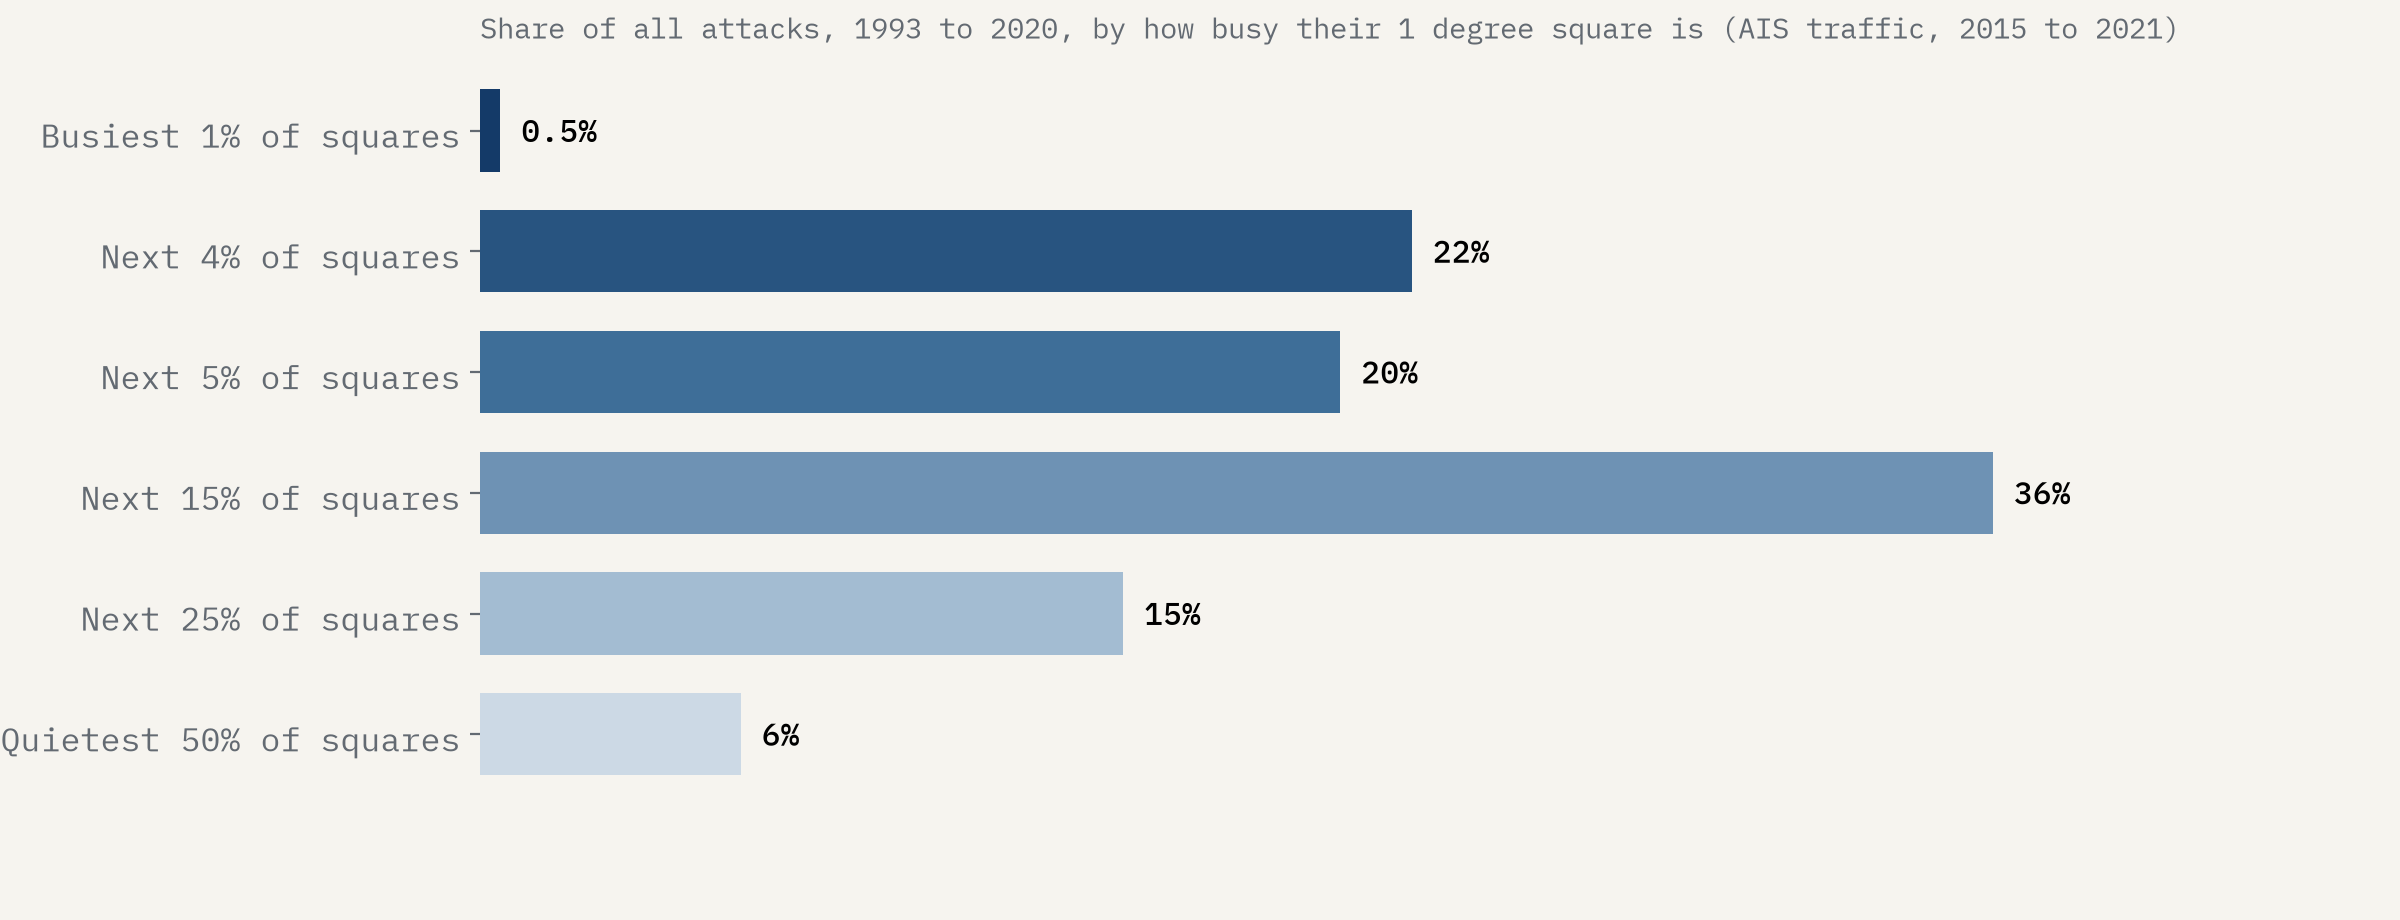
\includegraphics[width=\textwidth]{f_ship.png}
\caption{Share of attacks (1993 to 2020) by the traffic rank of their 1 degree square (AIS density, 2015 to 2021).}\label{fig:ship}\end{figure}

\subsection{Country context}
Of 6,788 attacks inside an EEZ with GDP data (1993 to 2019), 82\% were in countries with GDP per person below the world median of that year, and 75\% of those with a Corruption Perceptions Index score were in countries scoring below 35 of 100 (scores before 2012 multiplied by ten). Across 97 countries the rank correlation between total attacks and median GDP per person is $-$0.41 (Figure~\ref{fig:income}). This is consistent with work linking piracy to weak state capacity and economic opportunity \citep{daxecker,hastings}, but these simple associations cannot separate poverty from geography: many of the busiest straits and anchorages are in lower-income countries.

\begin{figure}[tbp]\centering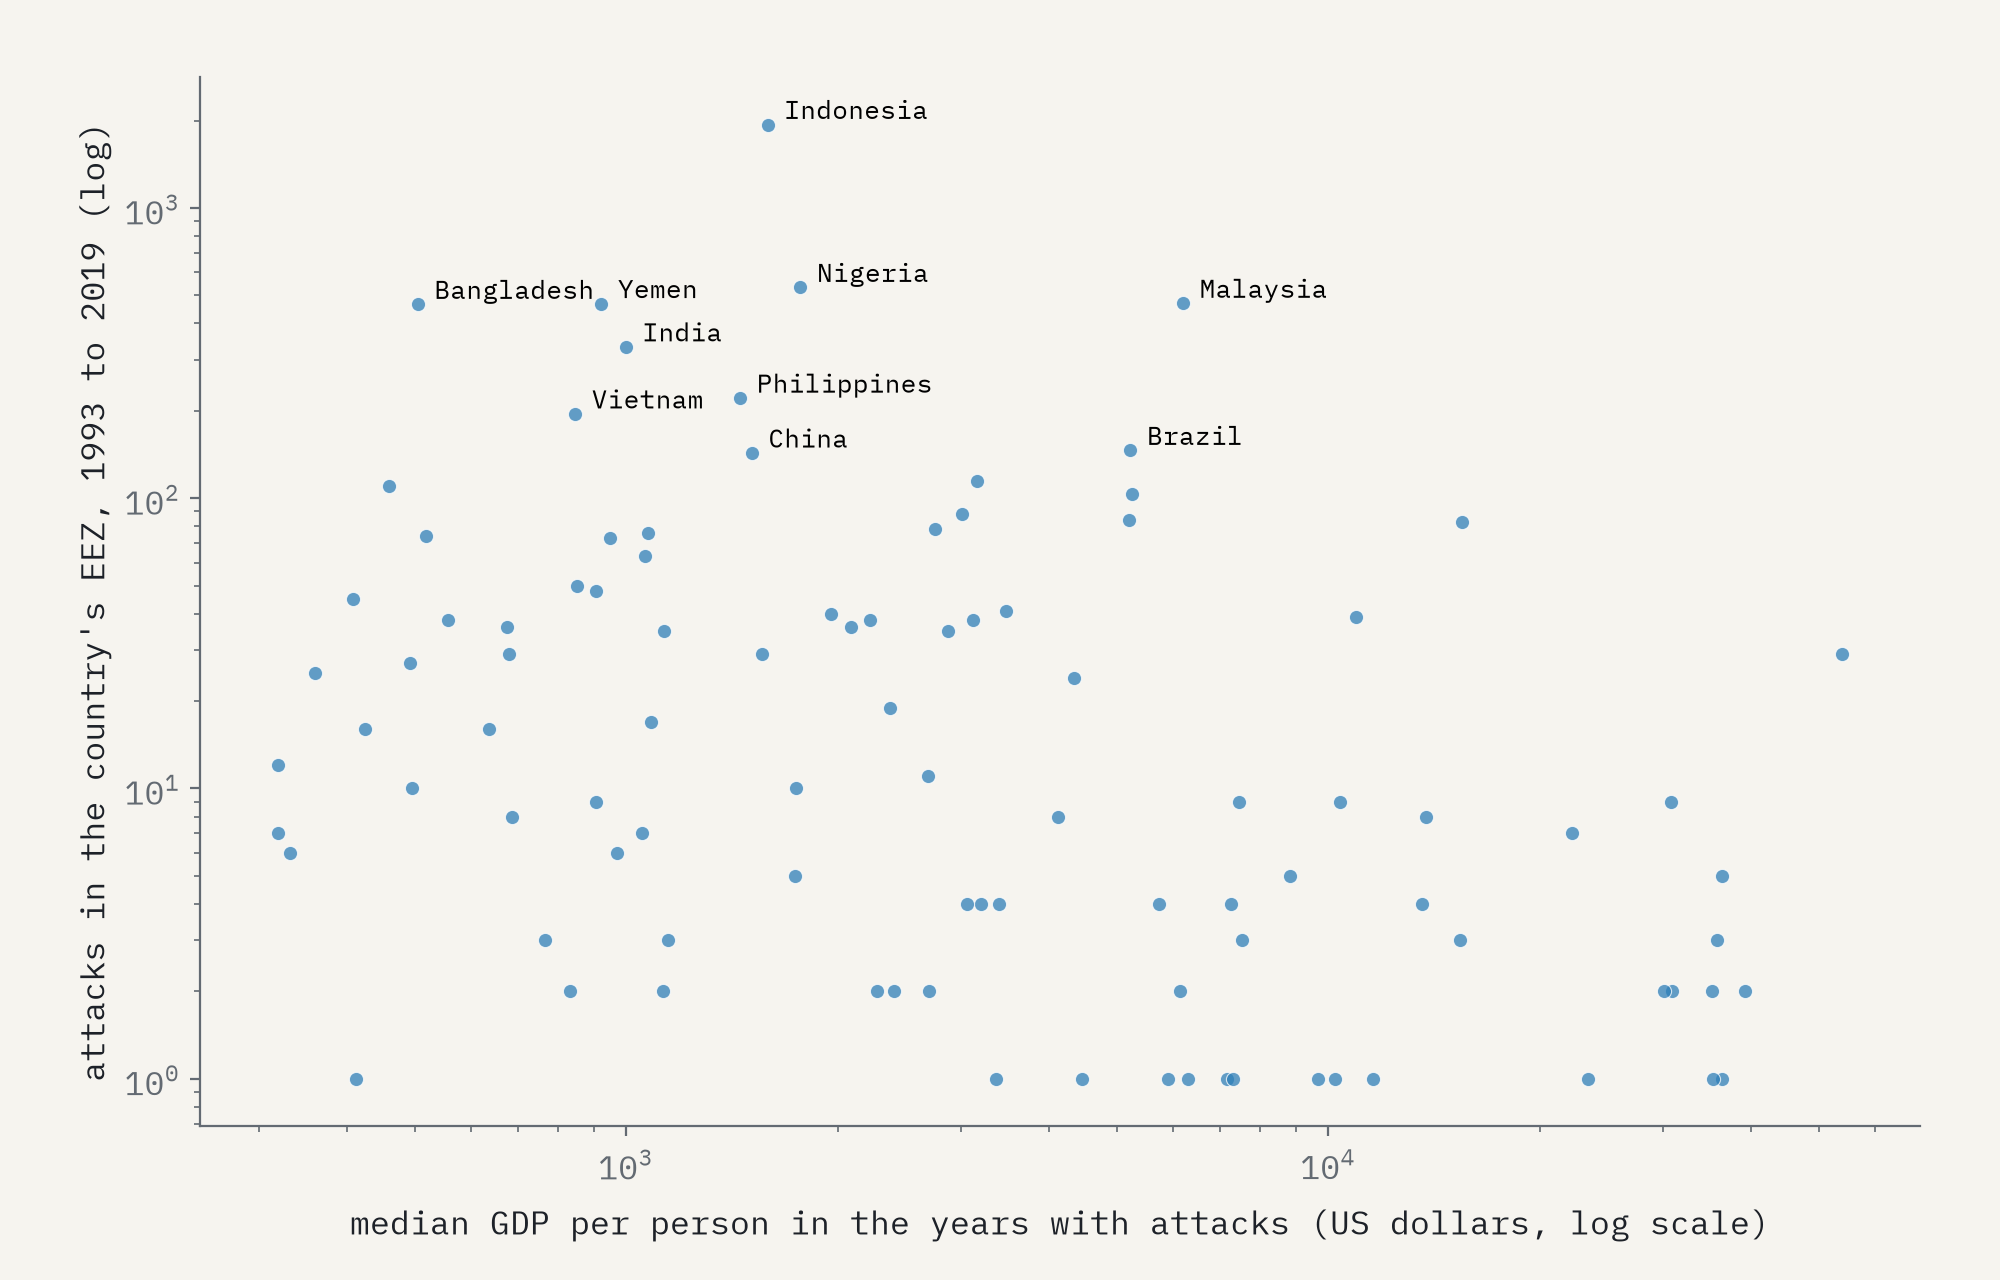
\includegraphics[width=.8\textwidth]{f_income.png}
\caption{Attacks in each country's EEZ, 1993 to 2019, against median GDP per person (country indicators from the database). Correlation, not cause.}\label{fig:income}\end{figure}

\subsection{Today: 2021 to 2026}
The IMB's counts (Table~\ref{tab:imb}, Figure~\ref{fig:today}) show a world total near 124 a year from 2021 to 2025. In 2025 the Singapore Strait recorded 80 incidents, 1.9 times its 2024 count and about as many as its mapped peak of 81 in 2015; it fell to 13 in January to September 2026 against 73 a year earlier. The Gulf of Guinea had 21 incidents in 2025 and 2 in the first nine months of 2026, Indonesia 12 and 6, and the Philippines 9 boardings in 2026. All 8 hijackings in January to September 2026 were by Somali pirates, who accounted for 94\% of crew taken hostage: ransom hijacking has returned to Somali waters on a scale not seen since 2012, when the database records 14 hijackings there.

\begin{figure}[tbp]\centering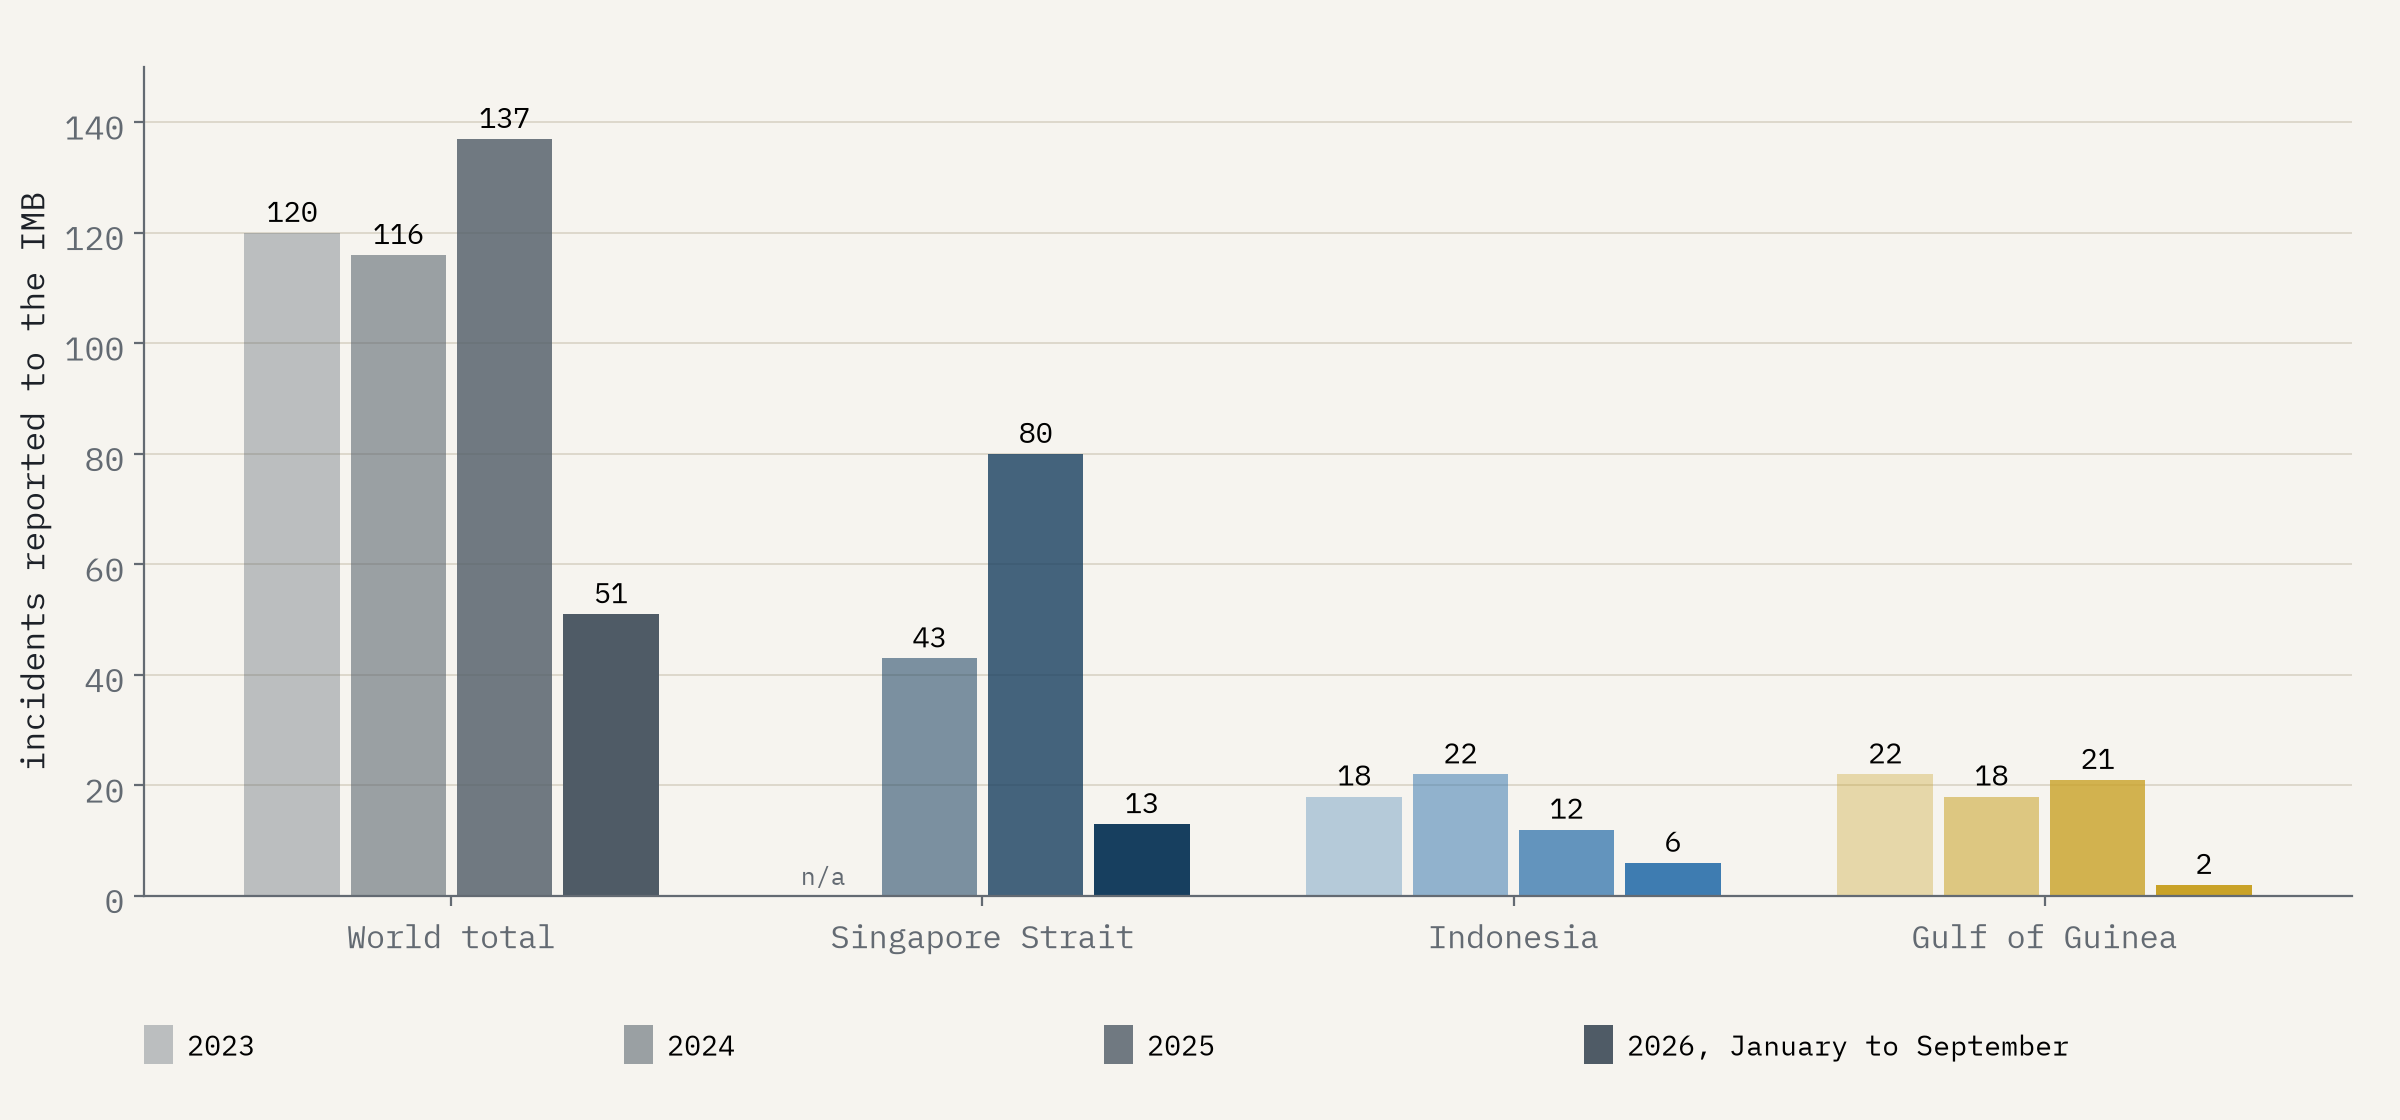
\includegraphics[width=\textwidth]{f_today.png}
\caption{IMB headline incident counts, 2023 to January to September 2026, for the world and the regions named in the releases.}\label{fig:today}\end{figure}

\begin{table}[tbp]\centering\small\caption{IMB headline incident counts, 2021 to January to September 2026, transcribed from IMB annual reports and press releases (blank where not given). Sources are listed with the data (data/imb\_recent.csv).}\label{tab:imb}\begin{tabular}{lrrrr}\toprule Period & World & Singapore Strait & Indonesia & Gulf of Guinea\\\midrule
2021 & 132 &  &  & \\
2022 & 115 &  &  & \\
2023 & 120 &  & 18 & 22\\
2024 & 116 & 43 & 22 & 18\\
2025 & 137 & 80 & 12 & 21\\
2025 Jan to Sep & 116 & 73 & 9 & \\
2026 Jan to Sep & 51 & 13 & 6 & 2\\
\bottomrule\end{tabular}\end{table}

\section{Limitations}
These are reported attacks. Under-reporting is widespread, especially of thefts from small craft, local vessels and fishing boats, and reporting varies with insurance, port politics and naval presence. The coding changes at 2015, when the source switches from the MAPPING data to IMB reports. Some anchorage attacks share a position copied from earlier incidents. Regions and eras are my own simple choices; other boundaries would shift some counts but not the broad pattern. The shipping layer covers 2015 to 2021, overweights areas with dense terrestrial AIS reception, and is matched to attacks from 1993 onwards. The IMB counts for 2021 to 2026 are headline figures from press releases, not points, and the 2026 figures cover nine months. The country indicators show associations only.

\section{Conclusion}
Piracy does not disappear; it relocates. Over three decades its centre of gravity moved from the South China Sea and Indonesia to the Strait of Malacca, then to the waters off Somalia, then to the Gulf of Guinea, and in 2025 to the Singapore Strait, with Somali hijacking returning in 2026. Each shift followed changes in enforcement and opportunity on some of the busiest shipping routes in the world.

\section*{Data and code availability}
The interactive map is at \url{https://maps.tristanhotham.com/piracy-hotspots/}. Data and code are at \url{https://github.com/Tristan-Hotham/piracy-hotspots} and archived with this paper at https://doi.org/10.5281/zenodo.23856383. Derived data are released under CC BY 4.0 and code under the MIT licence. The attack data are CC BY 4.0 \citep{benden}; the shipping density data are CC BY 4.0 \citep{wbships}.

\section*{AI statement}
I wrote the text, with drafting and editing assistance from Claude (Anthropic), which also helped prepare the analysis code. I reviewed and checked all text and results.

\begin{thebibliography}{9}
\bibitem[Benden et al.(2021)]{benden} Benden, P., Feng, A., Howell, C. and Dalla Riva, G. V. (2021) Crime at Sea: A Global Database of Maritime Pirate Attacks (1993 to 2020). \emph{Journal of Open Humanities Data} 7: 19. \url{https://doi.org/10.5334/johd.39}. Data: \url{https://github.com/newzealandpaul/Maritime-Pirate-Attacks}
\bibitem[Bueger(2015)]{bueger} Bueger, C. (2015) Learning from piracy: future challenges of maritime security governance. \emph{Global Affairs} 1(1): 33 to 42.
\bibitem[Cerdeiro et al.(2020)]{cerdeiro} Cerdeiro, D. A., Komaromi, A., Liu, Y. and Saeed, M. (2020) World Seaborne Trade in Real Time: A Proof of Concept for Building AIS-based Nowcasts from Scratch. IMF Working Paper 20/57.
\bibitem[Coggins(2012)]{coggins} Coggins, B. L. (2012) Global patterns of maritime piracy, 2000 to 2009: introducing a new dataset. \emph{Journal of Peace Research} 49(4): 605 to 617.
\bibitem[Daxecker and Prins(2013)]{daxecker} Daxecker, U. and Prins, B. (2013) Insurgents of the sea: institutional and economic opportunities for maritime piracy. \emph{Journal of Conflict Resolution} 57(6): 940 to 965.
\bibitem[Hastings(2009)]{hastings} Hastings, J. V. (2009) Geographies of state failure and sophistication in maritime piracy hijackings. \emph{Political Geography} 28(4): 213 to 223.
\bibitem[IMB(2026)]{imb} ICC International Maritime Bureau (2021 to 2026) Piracy and Armed Robbery Against Ships: annual and quarterly reports and press releases. \url{https://www.icc-ccs.org/}; 2026 release: \url{https://iccwbo.org/news-publications/news/maritime-piracy-incidents-remain-at-historic-lows-despite-somali-piracy-concerns/}
\bibitem[Liss(2011)]{liss} Liss, C. (2011) \emph{Oceans of Crime: Maritime Piracy and Transnational Security in Southeast Asia and Bangladesh}. Singapore: Institute of Southeast Asian Studies.
\bibitem[NGA(2026)]{asam} US National Geospatial-Intelligence Agency (2026) Anti-Shipping Activity Messages (ASAM). \url{https://msi.nga.mil/}
\bibitem[Natural Earth(2026)]{naturalearth} Natural Earth (2026) Admin 0 countries and populated places. Public domain. \url{https://www.naturalearthdata.com/}
\bibitem[Shortland and Vothknecht(2011)]{shortland} Shortland, A. and Vothknecht, M. (2011) Combating ``maritime terrorism'' off the coast of Somalia. \emph{European Journal of Political Economy} 27: S133 to S151.
\bibitem[World Bank(2013)]{worldbank} World Bank (2013) \emph{The Pirates of Somalia: Ending the Threat, Rebuilding a Nation}. Washington, DC: World Bank.
\bibitem[World Bank and IMF(2021)]{wbships} World Bank and IMF (2021) Global Shipping Traffic Density. CC BY 4.0. \url{https://datacatalog.worldbank.org/search/dataset/0037580}
\end{thebibliography}
\end{document}
